% Author: David Sanchez-Jacome

\chapter{Discussion and conclusions}\label{chap:discussion_and_conclusions} % (fold)

\section{Thermal crosstalk}\label{sec:thermal_crosstalk} % (fold)

\begin{figure}
	\begin{center}
		\includegraphics{figures/ch5-thermal_setup.pdf}
	\end{center}
	\caption{Setup of experiment used to measure the effect of thermal crosstalk on the iPronics chips.}\label{fig:ch5-thermal_setup}
\end{figure}

Thermal crosstalk is a major concern in silicon photonic integrated circuits (PICs) due to the high temperature sensitivity of photonic devices like Mach-Zehnder interferometers and microring resonators, which rely on precise refractive index control.
In densely integrated PICs, heat generated by thermal tuners can unintentionally affect neighboring components, leading to phase errors, wavelength shifts, and degraded performance.
Programmable PICs often pack numerous optical components and heaters (e.g., thermal tuners) into a compact area to achieve complex functionality.
Therefore, the proximity of these components means heat generated by one heater can unintentionally affect neighboring devices, causing unpredictable and undesired changes in their performance.
This issue increases power consumption, complicates thermal management, and reduces system stability and reliability, particularly as PICs scale in complexity.
To mitigate thermal crosstalk, strategies such as thermal isolation, active cooling, advanced control algorithms, and non-thermal tuning methods are explored to improve energy efficiency and ensure robust performance.
In particular, a silicon photonic platform implementing a set of underetched phase actuators optimized to contain the heat from the resistor within a small volume of air, leads to chips more resilient to thermal crosstalk aggression \cite{liu_thermo-optic_2022}.
Nevertheless, this design doesn't make the platform completely immune to this type of crosstalk.

During this thesis we have studied the effects of this thermal nonideality in the developed silicon photonic chips using underetch technology \cite{cem_thermal_2023, teofilovic_thermal_2024}.
To perform this study we synthesized a Micro Ring Resonator (MRR) in the mesh as this structure is very sensitive to thermal fluctuations (shown in Figure~\ref{fig:ch5-thermal_setup}).
The standard response of the MRR corresponds to a series of spectral notches occurring at wavelengths where the resonance condition is met:
\begin{equation}
	m\lambda = n_{eff}2\pi r
	\label{eq:ch5-ring_eq}
\end{equation}
where \(m\) is an integer value, \(n_{eff}\) is the effective group index of the propagating mode and \(r\) corresponds to the ring radius.
We then drove the thermal actuators of neighboring PUCs with high currents until the effect of thermal deviation was observed in the spectral response as depicted in Figure~\ref{fig:ch5-thermal_comp_ring1}.

\begin{figure}
	\begin{center}
		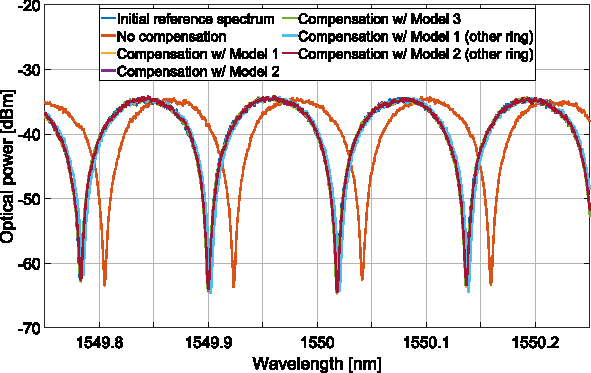
\includegraphics{figures/ch5-thermal_comp_ring1.pdf}
	\end{center}
	\caption{Response of an ORR circuit before and after the effects of severe thermal crosstalk and three proposed approaches to mitigate it.}\label{fig:ch5-thermal_comp_ring1}
\end{figure}

We observe that in the presence of this crosstalk aggressor the response of the circuit moves to the right as the effective refractive index \(n_{eff}\) increases with the temperature.
This leads the notches to shift to higher wavelengths while keeping the FSR constant.
Recall that this happened on a thermally controlled chip with isolated phase shifters, meaning that this effect is completely spurious.

If this undesired effect is to be mitigated, it has to be modeled first.
We considered two models: one based on the thermal diffusion of heat in a bulk material represented by a weighted summation of the phases \(\phi\) with the weight depending on
the distance \(d\) from the heat source \cite{jacques_optimization_2019} given by
\begin{equation}
	\Delta \lambda = \sum_i \left( p_1 e^{-p_2 d_i} + p_3 d_i + p_4 \right) \phi_i
	\label{eq:ch5-thermal_exp_fit}
\end{equation}
and another model based on a standard ridge regression that considers the driving phases of all the aggressor PUCs weighted by a train parameter
\begin{equation}
	\Delta \lambda = \sum_i a_i \phi_i + b
	\label{eq:ch5-thermal_ml_regressor}
\end{equation}
where in both cases \(p_i\), \(a_i\) and \(b\) are fitting parameters and where the regularization parameter was optimized using five-fold cross validation.

Both models were trained to minimize the root-mean squared error (RMSE) between the experimentally measured and the predicted wavelength shifts.
A large dataset is obtained measuring several neighboring PUCs driving currents and their subsequent phase shift: 80\% of the data was used for training and 20\% for testing.

\begin{figure}
	\begin{center}
		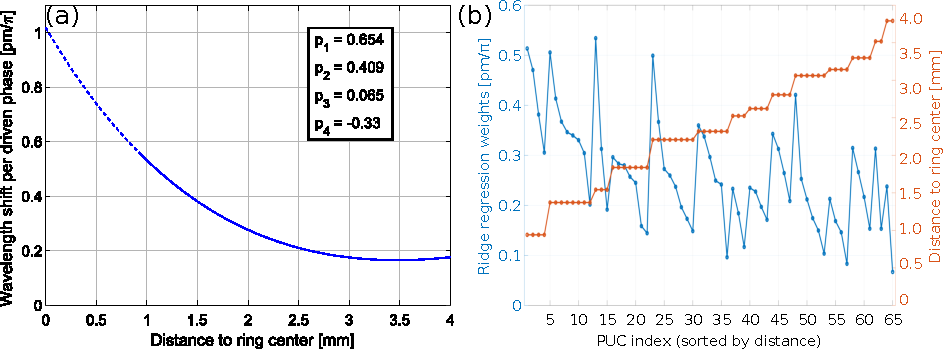
\includegraphics{figures/ch5-thermal_diffusion_correlation.pdf}
	\end{center}
	\caption{(a) Analytical  exponential decay model after fitting with optimal parameters shown in the box. (b) Weights found by ridge regression plotted alongside the distance to ring center for each PUC.
		The two are inversely correlated with \(\rho = -0.53\).
	}\label{fig:ch5-thermal_correlation}
\end{figure}

The analytical and data-driven models achieved 0.55 and 0.43 pm RMSEs, which resulted in testing RMSEs of 0.55 and 0.50 pm for, respectively.
Note that former model has four degrees of freedom, whereas the later 67 (66 weights and 1 bias).
The evolution of \(\Delta \lambda\) with distance is shown in Figure~\ref{fig:ch5-thermal_correlation} for the analytical model.
A major advantage of this model is that it can extrapolate to PUCs not considered in the experiment, providing valuable insight for future chip designs with more densely packed PUCs.
The weights found for the regressor model are presented in Figure~\ref{fig:ch5-thermal_correlation} where, although distance information was not fed to the regressor we observe an inverse correlation between the trained value and the distance to the regressor.
This method represents a black box approach that can be used when no information about the chip layout is available.

Finally, in order to validate the models created, we drove the 22 neighboring PUCs' cross phases (Fig.~\ref{fig:ch5-thermal_setup}) from \(0\) to \(2\pi\) and based on the models' predicted wavelength shift we counteracted it by applying the complementary phase shift \(\phi_c = 2 \pi(1-\frac{\Delta \lambda}{FSR})\) to one of the ring's actuators.
After the compensation, the initial and compensated notches were measured to be within \pm 0.5 pm.
Similar results were obtained when compensating a ring's shift using another ring's model as detailed in \cite{teofilovic_thermal_2024}.
This work paves the way to predicting and correcting the effects of severe thermal crosstalk in densely integrated PICs providing developers with principles to create lookup-table-based or active control loops to ensure reliability across chips for phase sensitive applications.
% section Thermal crosstalk (end)
\section{Optical computing}\label{sec:optical_computing} % (fold)

\begin{figure}
	\begin{center}
		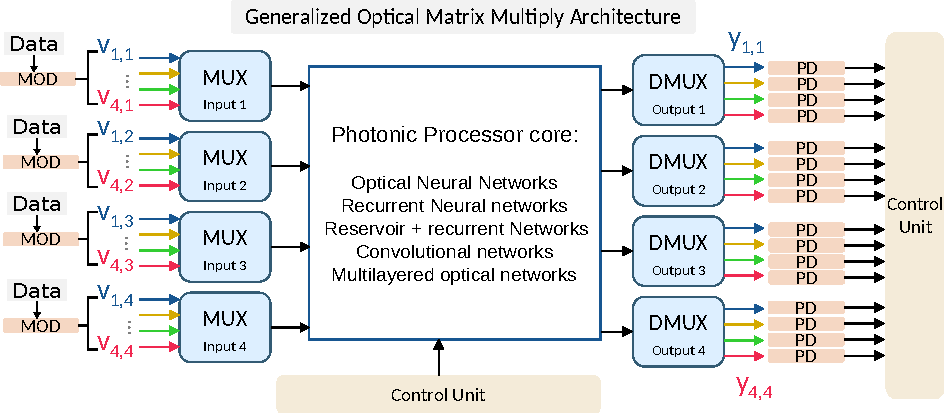
\includegraphics{figures/ch5-compute_schematic.pdf}
	\end{center}
	\caption{A schematic of an optical compute architecture based on a programmable PIC to perform multiply and accumulate operations.}\label{fig:ch5-compute_schematic}
\end{figure}

The promise of optical computing centers on its potential to transcend the limitations of conventional electronic computing by capitalizing on the inherent speed, parallelism, and energy efficiency of light.
With photons, computations could occur at the speed of light, enabling ultra-fast data processing and communication.
The capability to perform multiple operations simultaneously through different wavelengths or spatial paths could offer parallel processing power, particularly beneficial for matrix-heavy tasks in AI and machine learning.
Moreover, the analog nature of these optical solutions promise to consume less energy, reducing heat and power issues.

% - history
Although the interest for optical computing has been around for a few decades \cite{psaltis_holography_1990}, the recent AI and data center boom has reignited the race towards finding a faster and energy efficient solution to the increasing market demands based on this technology \cite{noauthor_could_2024}.
% - market reports
% - current approaches
Under this premise, the last decade has seen a proliferation of different approaches to come up with a viable optical approach to compete against GPUs \cite{zhu_space-efficient_2022,hu_diffractive_2024,zhu_space-efficient_2022,on_photonic_2022,feldmann_parallel_2021}.
As covered in chapter~\ref{chap:universal_unitary_operators}, optics provides an efficient platform to perform matrix multiplications, and thus it has been seen as an alternative candidate to help boost the massive amount of matrix multiplications required by AI training/inference while keeping the power bill on check.
In this section we present a study performed on the performance of a hypothetical optical compute architecture and its comparison with current GPU solutions.
We denote from the start that there is an intrinsic challenge when comparing both technologies as there is a significant gap between digital electronic solutions and optical ones.
First, the former has decades of maturity and competition on the latest foundry nodes that have yielded state-of-the-art performances.
Second, and most importantly, most attempts of comparison between the two often neglect the unavoidable optoelectronic conversion between optics (analog) and electronics (digital) that a feasible optical compute architecture should have.
This point in particular limits the scalability photonic computing solution due to SNR constraints on the bit resolution.
The following paragraphs take this into account and consider an optical matrix-multiply accelerator limited in size so that a minimal resolution of 8-bits can be achieved to make the comparison with a commercial GPU.

The architecture of an optical compute system based on MZI meshes to perform matrix calculations is presented in Figure~\ref{fig:ch5-compute_schematic}.
This solution is composed of three stages: an encoder, a generalized matrix multiplier section and a photodetection stage.
The first deals with moving the data from the digital electronics domain to the optical one by using a high speed modulator.
The second performs the matrix operation by transmission through the mesh with the matrix weights directly related to the driven phases as shown in chapter~\ref{chap:universal_unitary_operators}.
The third detects the signal, and moves it back to the electronic digital domain for subsequent processing.
One of the advantages of the optics approach is the use of WDM to increment the throughput of the network, therefore multiplexers and demultiplexers can be added in the first and third stages.
By doing this, more than one carrier can be multiplied by the active matrix.
The performance of GPUs is typically measured in terms of tera operations per second (TOPS) which measure the rate of \(10^{12}\) operations that can be carried out by the electronics card per second.
In the case of the optical architecture in Fig.~\ref{fig:ch5-compute_schematic} this metric is defined by \eqref{eq:ch5-compute_tops}

\begin{equation}
	TOPS = \frac{N^2 C}{\frac{1}{K f_{ps}}+\frac{1}{n_{\lambda}f_{mod}}} \label{eq:ch5-compute_tops} \end{equation}

Where \(N\) is the size of the unitary operator implemented by the photonic mesh, \(C\) is the number of cores, \(K\) is the batch size (typically large for inference tasks), \(f_{PS}\) is the operating frequency of the phase shifter, \(n_{\lambda}\) is the number of multiplexing wavelengths and \(f_{mod}\) is the encoding modulator speed.

\begin{figure}[h]
	\begin{center}
		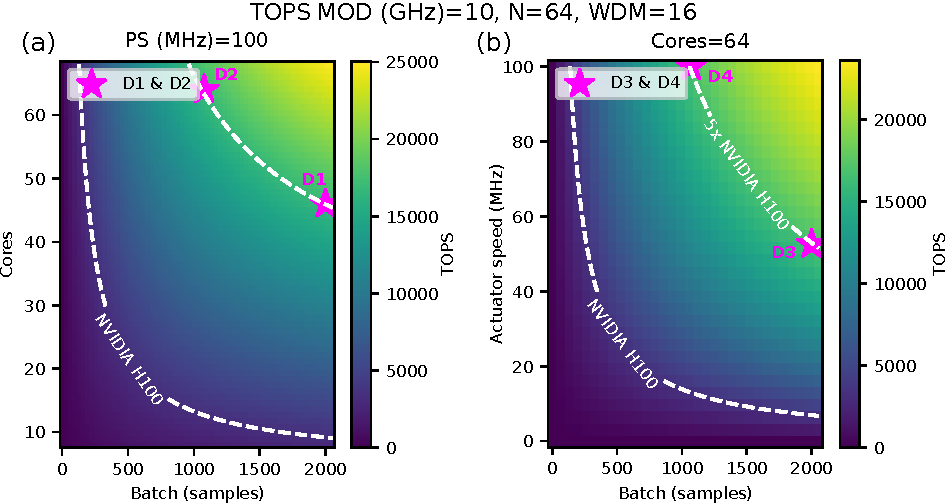
\includegraphics{figures/ch5-compute_tops_batchs.pdf}
	\end{center}
	\caption{TOPS of an optical compute architecture based on MZI meshes and exploiting WDM, multicore and high-speed phase actuators techniques.
		The white contours show the performance for different H100 Nvidia GPUs for reference.
	}\label{fig:ch5-compute_tops}
\end{figure}

The resulting TOPS obtained by sweeping $C$ (\# of cores) with $K$ (batch size) and $f_{PS}$ (phase shifter frequency) with $K$ (batch size) are presented in Figure~\ref{fig:ch5-compute_tops} (a) and (b), respectively.
Note that the white contours also show the TOPS performance of an Nvidia H100 tensor core GPU and a 5x improvement of this metric.
For an optical matrix multiply accelerator to be a viable competitor of conventional electronic GPUs, at low-precision (8 bits) inference workloads, it must at least yield a five-fold improvement with respect to the latter.
Because of this we have chosen four different designs (D) of possible architectures as seen in Table~\ref{tab:ch5-compute_tops}.
To perform this comparison with respect to the H100 system we have chosen a set of fixed ambitious metrics such as a unitary operator of size 64, 16 wavelength carriers \cite{noauthor_cw-wdm_nodate} and a high speed on chip modulator of 10 GHz.
We have chosen 64 as the maximum size of the matrix as our models show that's the maximum size to achieve 8 bit of resolution in an optimized system \cite{ward-foxton_optical_2021}.
This resolution is directly limited by the losses introduced by the chip.

\begin{table}
	\centering
	\caption{Different optical matrix-multiply architectures required to reach 5x performance improvement compared to an Nvidia H100. Both architectures are compared at 8-bit precision performance}\label{tab:ch5-compute_tops}
	\begin{tabular}{|c|c|c|c|c|}
		\hline
		Architecture & \# of Optical Cores & Actuator frequency (MHz) & Batch size & H100 comparison \\
		\hline
		D1           & 46                  & 100                      & 2000       & 5x              \\
		\hline
		D2           & 64                  & 100                      & 1080       & 5x              \\
		\hline
		D3           & 64                  & 52.6                     & 2000       & 5x              \\
		\hline
		D4           & 64                  & 100                      & 1070       & 5x              \\
		\hline
	\end{tabular}
\end{table}

The results show that even for a relatively large batch size (typical values are around 128 due to memory bandwidth limitations \cite{noauthor_llm_2023}) the systems need a very fast phase shifter with a rise time in the sub ns range and a massive multicore approach (> 46) to achieve a performance 5 times the one of a single H100 card \cite{noauthor_nvidia_nodate}.
When we compare this with a multicore GPU systems such as the DGX H100 system that contains 8 H100 cards with a performance of 32 petaOPS (i.e., 9.7x that of an H100 card) the picture becomes grimmer \cite{noauthor_nvidia_nodate-1}.

The pros of the optical solution are the high encoding frequency of optical modulators and low propagation latency given by the propagation of light in silicon.
The cons, however, overshadow the latter because on one hand the losses and bulkiness of silicon photonics limit the maximum operator size which in turn means that large matrices have to be split in numerous tiles to be optically implemented.
On the other hand, the relatively slow phase changing effect (constrained in turn to yield the lowest losses possible) severely limits the refresh speed of weights in the matrix and impacts negatively the system's performance.
Another big problem is the need to move data from the digital domain to the analog and back to the digital \cite{meech_data_2023} which introduces costly conversions and limits the resolution.
These are the reasons we observe the need of a massive multicore, multiwavelength architecture to the performance of a single H100 card.
Of course, these solutions involve non-trivial technical challenges, don't scale well and can't match the metrics of their electronic multicore counterparts such as the DGX H100 or the NVL72.
Perhaps this is the reason several optical compute startups have changed their value propositions and moved to data movement instead.
It's true that current AI boom required faster, cheaper and more energy efficient solutions that can enable the democratization and application build-up of AI technology.
The evidence suggests that the current systems' bottleneck is not on the compute side, but rather on the enormous data flow requirements of AI \cite{cole_optical_2021} and this is where this kind of silicon photonics MZI meshes stand higher chances to find a killer app.
For pure photonic computing to become competitive, researchers must find additional avenues in high-speed (>30GHz) time domain computing capabilities in order to truly leverage on the very high bandwidth capabilities of optics \cite{tsakyridis_photonic_2024}.
We must recall, however, that an all-optical solution is not realistic making an optoelectronic approach the only option left, for which the aforementioned tradeoffs must be considered seriously.
% section Optical computing (end)
\section{Conclusions}\label{sec:conclusions} % (fold)

% - The achievements of this thesis
% - Full tech stack system
% - Summary of applications with refs
This dissertation covers the developments made to design, fabricate and assemble a multipurpose programmable photonics platform powered by a reconfigurable silicon on insulator chip.
The activities carried out during this research touched different points of the technology stack with special emphasis on the layout design of the chip, the control electronics and the software control layer to interact with the silicon core.
As a result of three years of work and a team of enthusiastic hardworking engineers and scientists the iPronics first-generation Smartlight platform was made commercially available in December 2022 and publicly presented at OFC 2023.
The published applications demonstrated on the same commercial platform span several fields: microwave photonics \cite{perez_multipurpose_2017, perez-lopez_general-purpose_2024,catala-lahoz_self-configuring_2023}, topological photonic arrays \cite{on_programmable_2024,hashemi_non-hermitian_2024}, beamforming networks \cite{perez-lopez_programmable_2018}, optical computing architectures \cite{ashtiani_photonic_2023,ashtiani_universal_2024,ashtiani_programmable_2024}, datacom networking \cite{xie_software-defined_2024}, among others.
Some of these demonstrators have been the first of their kind and therefore have been published in world-class journals.
Moreover, several groups of researchers around the globe are currently prototyping and working on new applications using this platform.

% - Emphasis on Software stack and capabilities
% - Synthesis and configuration algorithms
% - Python API
% - Fast API
Although the first months of this thesis focussed on chip layout and design, the big majority of the work carried out was related to the software control layer and demonstration of applications.
As covered in chapter 3, the activities dealt with the creation of several abstraction layers on top of the silicon chip to create a human-readable interface that would allow configuring and synthesizing different applications on the chip.
The software stack encompasses the orchestration of the control and monitoring electronics, a temperature controller (TEC) and other peripherals through a logic unit (LU) that hosts the algorithms and routines to boot and drive the system.
Among the key routines stored here we found the calibration, the manual configuration and automatic configuration algorithms, and hardware maintenance processes.
A special emphasis was made on the manual and automatic configuration where the former relies on automatically retrieved cached calibration information for the different PUCs and the latter implements an additional graph-based abstraction layer to find the optimum circuit for a given high-level request and a figure of merit.
The algorithms are accessible to the user via a Python API which, alongside other auxiliary tools like core, power and spectrum monitors, serves as a powerful yet user-friendly SDK to prototype several applications.
The Python API serves as a way to interact directly with the standalone system much like the Arduino IDE \cite{noauthor_software_nodate} or Vivado Suite \cite{noauthor_amd_nodate} bridge the human with the microcontroller or FPGA, respectively.
If the system is meant to be used in conjunction with other systems and all of them have to be controlled synchronously by an operator (e.g., a lab environment), a FAST-like API \cite{noauthor_fastapi_nodate} is more sustainable for application testing and deployment.

% - Prospects of the field
% - multipurpose for research: Nokia bell labs papers
% - volume consumption requires application specific
% - Potential killer applications volume
Looking forward to the future of this technology platform we foresee that it will continue to be a key enabler of new application prototyping.
While the standard way of prototyping new applications requires the design and fabrication of ASPIC chips, the multipurpose platform documented in this thesis offers a cheaper and faster alternative to do something similar on a configurable chip.
We must recall, however, that the speedup of development cycles comes with the tradeoff of slightly worse specs due to spurious effects in mesh-based systems.
In most cases though, these effects can be counteracted using the built-in software layer and user-defined routines.
In addition, hardware improvements are becoming progressively reachable.
Reducing the insertion loss for wideband operation \times 4 times, while keeping low first-order crosstalk levels, is already attainable with optimized building blocks.
Nevertheless, for these devices to be deployed in volume, an application with a sizeable market needs to be found first through the prototyping and test trials R\&D groups are currently running.
The existence of a potential "killer app" should be determined in the upcoming years.
A couple of good ways to facilitate the quest for new applications might be open sourcing the chip architecture and instruction set as well as defining standards on the API level so that more researchers can contribute and lead to the formation of a community such as the RISC-V project \cite{noauthor_risc-v_nodate}.
In the meantime we forecast that in the short and mid terms most companies will focus on programmable ASPIC solutions for fields like computing \cite{noauthor_akhetonics_nodate}, chip-to-chip interconnects \cite{noauthor_celestial_nodate,noauthor_passage_nodate}, optical circuit switching \cite{noauthor_ipronics_nodate, noauthor_salience_nodate}, LiDAR \cite{noauthor_opa_2021}, among others.
As these solutions become more pervasive, their need for testing and prototyping using multipurpose PICs is expected to grow in the long run either as standalone development systems or IP blocks.

% section Conclusions (end)
\section{Future work}\label{sec:future_work} % (fold) 
\subsection{Photonic hardware defined language}\label{sub:phdl} % (fold)

Hardware Description Languages (HDLs) like Verilog and VHDL are essential for designing and simulating digital circuits, enabling engineers to model complex hardware systems at various abstraction levels.
HDLs provide a platform for describing Register-Transfer Level (RTL) designs, allowing for precise control over data flow, timing, and hardware behavior.
Their use is critical in modern workflows as they offer the ability to simulate and verify designs before physical implementation \cite{katz_contemporary_2005}.
Furthermore, HDLs bridge the gap between high-level design concepts and physical hardware by enabling synthesis into gate-level structures and deployment onto chips or programmable logic devices \cite{pedroni_circuit_2004}.
This capability makes them indispensable for both rapid prototyping and large-scale production.

FPGAs synthesize HDL code by transforming high-level hardware descriptions into configurations for the FPGA's programmable logic.
The process begins with synthesis tools, which compile HDL code into a netlist of logic gates optimized for resources and timing.
This netlist is then mapped to the FPGA's architecture, assigning Look-Up Tables (LUTs), flip-flops, and other primitives.
The place-and-route stage determines the physical arrangement and connections within the FPGA, ensuring signal integrity.
Finally, the design is converted into a bitstream file, which programs the FPGA to implement the specified circuit.
Tools like Xilinx Vivado \cite{noauthor_amd_nodate} and Intel Quartus \cite{noauthor_fpga_nodate} streamline this process, enabling efficient realization of custom hardware designs.

The case for a Photonic Hardware Description Language (PHDL) is very similar to its electronic counterpart.
On one hand, we have a set of primitives (e.g., tunable couplers, modulators, photodetectors, splitters, etc.) that can be connected with each other to create complex circuits.
And on the other hand we have either a multipurpose mesh that can connect all these elements together (in an FPPGA system) or a set of waveguide connectors that help to place and route the optical components (in an ASPIC system).
If such circuits can be described in terms of a netlist such electronic ICs then they could also be described/synthesized using a higher abstraction level, i.e., a PHDL, and interconnected using the same principles \cite{lee_algorithm_1961}.
Such abstraction layer has to consider the non-trivial aspect that photonic ICs are analog instead of digital, which introduces new design constrains.
Of course this also means that a synchronous description of the hardware behavior such as RTL would not be of much use for PHDLs.
As PICs circuits are in many cases based on interferometry and phase control, a PHDL implementation would need to strongly enforce length equalization and path length difference to work appropriately.
The synthesis of PHDL code should also minimize waveguide lengths and crossings as they introduce critical loss/phase and optical crosstalk parasitics, respectively.
Attempts in the electronic field to implement analog HDLs based on modern languages such as Python \cite{fritchman_integrated_2023} should be used as reference.
A first implementation of PHDLs could focus on synthesizing and connecting different primitives in a multipurpose mesh such as the one presented in Chapter~\ref{chap:applications_using_fppgas} where path lengths are discrete by design.
The abstraction could then be upgraded and generalized to the design of complex ASPICs following the principles of \cite{lee_algorithm_1961} and taking into account the constraints of optics.

% subsection Photonic hardware defined language (end)
\subsection{Amplification}\label{sub:amplification} % (fold)

% The problem is losses from silicon
Losses in silicon photonics chips significantly impact performance and efficiency.
These losses arise from factors like waveguide sidewall roughness, mode mismatches and material absorption.
Mitigation strategies include advanced fabrication techniques, optimized waveguide, components and coupler designs.
In spite of this, as PICs become larger the insertion losses build-up up to the point where their use in commercial applications becomes very difficult.
% Some kind of compensation is needed for which SOA are ideal or edwas
For this reason, some kind of compensation is needed to retrieve the signal to functional levels.
The perfect candidates for the compensation are semiconductor optical amplifiers (SOA) as they are mature, can be miniaturized and produced in volume.
Erbium-doped waveguide amplifiers (EDWA) promise to be a good alternative once they reach maturity and volume manufacturing \cite{noauthor_edwatec_nodate,liu_photonic_2022}.
% Active introduces nonidealities
In any case, the introduction of active elements in the system will also bring nonidealities into play.
The effects of the latter have been studied in microwave photonics \cite{sanchez_modeling_2021}, telecom \cite{bonk_soa_2018} and datacom networks \cite{o_duill_estimation_2017, way_technical_2014,maharry_integrated_2023}.
The studies show that it's important to develop techniques to suppress waveform distortion when driving the active elements \cite{masumoto_approach_2022}.
Among the key metrics that will have to be optimized when amplifiers are introduced to compensate chip losses we have: signal-to-noise ratio (SNR), bit-error ratio (BER) and transmitter dispersion eye closure (TDECQ), for PAM4 signals.
Different types of amplifiers will need to be optimized and compared between each other to ensure the highest signal quality \cite{st-arnault_performance_2024} at the system's output.
If the application handles WDM signals then the flatness of the chip's transmission response and the amplifier's spectral mask will need to co-designed and refined ensemble.

% subsection Amplification (end)
\subsection{Circuit aware calibration}\label{sub:circuit_aware_calibration} % (fold)

As covered in Chapter~\ref{chap:universal_unitary_operators}, when synthesizing phase-sensitive circuits in the mesh, the spectral response of the hardware doesn't match with the simulation results \cite{on_programmable_2024,sanchez_gomariz_scalability_2024}.
It was observed that although hardware and simulation match well for circuits depending on coupling factor \( k\) alone (e.g., interconnects, beamsplitters), there are mismatches with circuits that imply interferometry (phase-dependency) such as filters and multiport interferometers \cite{zand_effects_2020}.
This led to the formulation of a new model for the PUC presented in Section~\ref{sub:updated_puc_model} to consider the passive phase introduced by PUC connections.
In Chapter~\ref{chap:universal_unitary_operators}, we covered how these phases could be calibrated for super PUC structures, however other structures such as ring arrays and IIR/FIR filters will still require a calibration routine of their own to work correctly.
This brings two options to the table as follow-up actions: either a calibration routine needs to be run for each phase-sensitive circuit, which encompass a very large subset of structures, or the \(\phi^u_p\) and \(\phi^l_p\) values of each PUC need to be characterized beforehand, so they can be compensated in every circuit.
The first approach is rather straightforward as we only need to make sure that a phase offset is added to individual interferometric structures for them to match their expected response as done in \cite{on_programmable_2024}.
The problem with this approach is that it requires to create a routine for each different circuit as the passive phases involved in each one will be different.
The second approach requires finding enough independent equations (i.e., circuits) so that \(\phi^u_p\) and \(\phi^l_p\) can be determined for the entire mesh solving a linear equations' system.
With this information, any phase-sensitive circuit can be compensated automatically during the synthesis without the need of a per-case calibration.
The issue with this option is that finding enough equations to identify these variables can be a non-trivial task and requires the implementation of a fully automated process that can be used in several circuits to infer phase drifts in terms of different observable variables.
A third, and more complicated approach is to use on-chip photodetectors, so the user can implement self calibration algorithms such as resonance positioning using the inputs from these PDs.
The problem with this approach is that it introduces more losses and significant fabrication complexity.
In most cases, the use of a phase-sweep routine (approach 1) might be enough and faster to implement to start prototyping the application of interest.
Nevertheless, as this kind of recirculating meshes are ported to other platforms \cite{kim_programmable_2023,zhang_compact_2024,zhang_programmable_2025} and the arrays grow larger this issue will have to be addressed.
% subsection Circuit aware calibration (end)

% section Future work (end)
% chapter Discussion and Conclusions (end)
